\documentclass[addpoints ]{exam}

\printanswers
\usepackage{amssymb, amsmath, amsfonts}
\usepackage{geometry}
\usepackage{graphicx}
\usepackage{tikz}
\usetikzlibrary{calc}
\usepackage{multirow,array} % for payoff matrix formatting
\usepackage{hyperref}
\usepackage{xcolor}
\hypersetup{
  colorlinks = true,
  linkcolor  = gray,
  urlcolor   = blue
}

\geometry{left=1.0in,right=1.0in,top=1.0in,bottom=1.0in}
\pagestyle{headandfoot}
\lhead{EC327 Game Theory}
\chead{Homework 6}
\rhead{Fall 2025}
\runningheadrule

\title{
    \textbf{Econ 327: Game Theory} \\ 
    Homework $\#6$
    }
\author{University of Oregon}
\date{Due: Nov. 19$^{th}$}

% exam-type question formatting
\renewcommand{\thequestion}{\textbf{Q\arabic{question}}}
\bracketedpoints

\begin{document}

\maketitle

\begin{center}
  \gradetable[h][questions]
\end{center}

\vspace{0.5in}

\begin{center}
  \textbf{For homework assignments:}
\end{center}

\begin{itemize}

%  \item DO NOT write your name:
%  this assignment will be graded anonymously. 
%  If you want to, you can include your student ID instead.

  \item Complete \textit{all} questions and parts.
  % I will select one question at random to be graded
  % according to the rubric on Canvas.

  \item You will be graded on not only the content of your work
    but on how clearly you present your ideas.
    Make sure that your handwriting is legible.
    Please use extra pages if you run out of space 
    but make sure that all parts of a question 
    are in the correct order when you submit.

  \item You may choose to work with others,
  but everyone must submit to Canvas individually.

  Please include the names of everyone who you worked with 
  below your own name.
 
\end{itemize}

\vspace{1.0in}

\makebox[.6\textwidth]{Name\enspace\hrulefill}

\vspace{0.5in}

\begin{center}
  \fbox{\fbox{\parbox{5.5in}{\centering
  \textbf{Note:}
  All Questions are adapted from problems in  
  Dixit, Skeath and Reiley, \textit{Games of Strategy}, Fourth Edition. 
  }}}
\end{center}

\newpage

\begin{questions}

%------------------------------------------------------------------%

\newpage

\question
Consider a subsistance economy where each farmer has their own plot of land.
The yield of each plot of land depends on the local weather conditions.
With 50\% probability, there are good growing conditions and a plot yields 
100 bushels of yams.
On the other hand, there is a 50\% chance that growing conditions are bad,
in which case the plot only yields 36 bushels.

Suppose that all farmers are risk-averse,
and they each have a utility function $u(x) = \sqrt{x}$ 
for any $x$ number of bushels they consume.

\begin{parts}
  \part[4]
  Solve for one farmer's expected utility for one harvest year.
  How many bushels would they have to recieve for certain
  to receive the same amount of utility?
  \begin{solution}
    \begin{align*}
      EU & = p(Good) \times u(100) + p(Bad) \times u(36) \\
         & = \frac{1}{2} \times \sqrt{100} + \frac{1}{2} \times \sqrt{36} \\
         & = 8
    \end{align*}
    To get the same amount of utility from a certain amount of consuption,
    the farmer would have to get $x=64$ bushels, so that $u(64) = 8$.
  \end{solution}
  \part[4]
  Now suppose that there are two farmers who own separate plots
  where the probability of good or bad growing conditions on each farmer's plot
  are completely independent of each other.
  Suppose that they can agree to the following deal.
  Regardless of their respective luck, 
  they will always pool their harvests and then split them equally.
  What are the probabilities of each of the four possible luck combinations?
  Solve for the expected utility to either farmer under this deal.
  \begin{solution}
    If conditions are truly independent on each plot, then the probability of each outcome is 1/4.
    \begin{itemize}
      \item With $p=1/4$, Good, Good: total harvest = 100 + 100
      \item with $p=1/4$, Good, Bad: total harvest = 100 + 36
      \item with $p=1/4$, Bad, Good: total harvest = 36 + 100
      \item with $p=1/4$, Bad, Bad: total harvest = 36 + 36
    \end{itemize}
    The expected utility for either farmer is then:
    \begin{align*}
    EU & = 0.25\sqrt{\frac{200}{2}} + 0.5\sqrt{\frac{136}{2}} + 0.25\sqrt{\frac{72}{2}} \\
       & = 2.5 + 0.5\sqrt{68} + 1.5 \approx 8.12
    \end{align*}
  \end{solution}
  \part[4]
  Would it make sense for a farmer to take this deal?
  How many bushels of their harvest would a farmer be willing to pay
  for an insurance policy that guarantees the pooled harvests?
  Explain in your own words.
  \begin{solution}
    The certainty equivalent of the lottery when farming alone in part (a) is 64 bushels.
    The certainty equivalent of the harvest-sharing deal in part (b) is $8.12^2\approx 65.98$ bushels.
    So a risk-averse farmer likes the sharing outcome better and would be willing to pay about 1.98 bushels
    of their harvest to join the harvest sharing.
  \end{solution}
\end{parts}

\newpage

%------------------------------------------------------------------%

\question
A local charity has been given a grant to serve free meals to the homeless in its community, but it is worried that its program might be exploited by nearby college students, who are always on the lookout for a free meal.
Both a homeless person and a college student receive a payoff of 10 for a free meal.
The cost of standing in line for the meal is 
$t^2 / 250$ for a homeless person and 
$t^2 / 160$ for a college student,
where t is the amount of time in line measured in minutes.
Assume that the staff of the charity cannot observe the true type of those coming for free meals.
Also assume that the payoff of not eating a meal (and not waiting) is always zero.

\begin{parts}
  \part[4] What is the minimum wait time that will keep college students away?
  \begin{solution}
    40 minutes
  \end{solution}
  \part[4] What is the maximum wait time until homeless people also leave the line?
  \begin{solution}
    50 minutes
  \end{solution}
  \part[4] 
  After a while, the charity finds that it can successfully identify 
  and turn away college students half of the time.
  College students who are turned away receive no free meal,
  still have to wait in line,
  and, further incur a cost of 5 for their time and embarrassment.
  Will the partial identification of college students 
  reduce or increase the answer in part (a)? 
  Explain.
  \begin{solution}
    \begin{align*}
      EU_{\text{Student}}(Waiting) & = 0.5(10 - \frac{t^2}{160}) + 0.5(-5 -\frac{t^2}{160}) \\
      EU_{\text{Student}}(Leaving) & = 0
    \end{align*}
    Now college students will be turned away as long as $t<20$.
    Compared to part (a), partial identification \textbf{decreases}
    the expected utility of waiting in line,
    so it takes less of a wait time to deter them.
  \end{solution}

\end{parts}

%------------------------------------------------------------------%

\newpage

\question
Consider a game between a union and the company that employs the union
membership. The union can threaten to strike (or not) to get the company to
meet its wage and benefits demands. When faced with a threatened strike, the
company can choose to concede to the demands of the union or to defy its threat
of a strike. The union, however, does not know the company’s profit position
when it decides whether to make its threat; it does not know whether the
company is sufficiently profitable to meet its demands—and the company’s
assertions in this matter cannot be believed. Nature determines whether the
company is profitable; the probability that the firm is unprofitable is $p$.

The payoff structure is as follows: (i) When the union makes no threat, the
union gets a payoff of 0 (regardless of the profitability of the company). The
company gets a payoff of 100 if it is profitable but a payoff of 10 if it is
unprofitable. A passive union leaves more profit for the company if there is
any profit to be made. (ii) When the union threatens to strike and the company
concedes, the union gets 50 (regardless of the profitability of the company)
and the company gets 50 if it is profitable but -40 if it is not. (iii) When
the union threatens to strike and the company defies the union’s threat, the
union must strike and gets -100 (regardless of the profitability of the
company). The company gets -100 if it is profitable and -10 if it is not.
Defiance is very costly for a profitable company but not so costly for an
unprofitable one.

\begin{parts}
  \part[4] 
  What are the best responses of the profitable and unprofitable company types
  when the union uses the pure threat to strike unless
  the company concedes to the union’s demands?

  \begin{solution}
    \begin{align*}
      \text{If unprofitable:} &
      \begin{cases}
        EU_C(\texttt{Defy}) = -10 \\
        EU_C(\texttt{Concede}) = -40 \\
      \end{cases}
      \text{, always Defy} \\
      \text{If profitable:} &
      \begin{cases}
        EU_C(\texttt{Defy}) = -100 \\
        EU_C(\texttt{Concede}) = 50 \\
      \end{cases}
      \text{, always Concede} \\
    \end{align*}
  If p is too high for threat to be worth it for Union,
  the SPNE is \{\texttt{No Threat}, (\texttt{Defy} if unprofitable, \texttt{Defy} if profitable)\}.

  If p is low enough for threat to be worth it,
  the SPNE is \{\texttt{Threat}, (\texttt{Concede} if unprofitable, \texttt{Defy} if profitable)\}.
  \end{solution}


  \part[4] Suppose that the union sets up a situation in which there is some
  risk, with probability $q < 1$, that it will strike after the company defies
  its threat.
  This risk may arise from the union leadership’s imperfect ability to keep the
  membership in line.
  Draw an extensive form game tree.

  \begin{solution}
    \begin{center}
      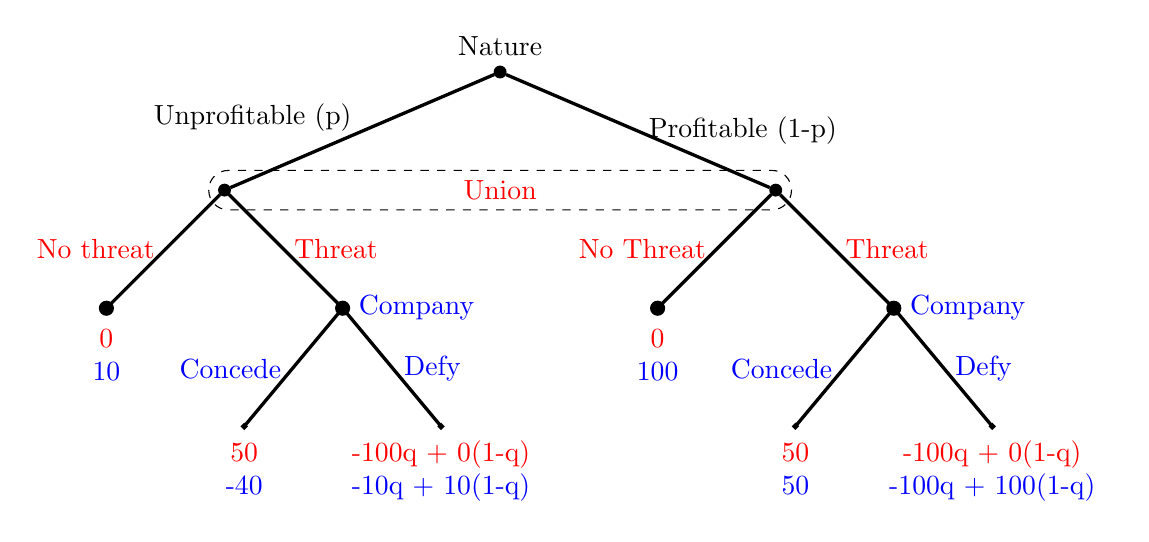
\begin{tikzpicture}[edge from parent/.style={draw, very thick}]
    \tikzstyle{solid node}=[circle,draw,inner sep=1.5,fill=black]
    \tikzstyle{hollow node}=[circle,draw,inner sep=.25]
    \tikzstyle{level 1}=[level distance=15mm,sibling distance=7cm]
    \tikzstyle{level 2}=[level distance=15mm,sibling distance=3cm]
    \tikzstyle{level 3}=[level distance=15mm,sibling distance=2.5cm]
    \tikzstyle{pruned edge from parent}=[draw, very thick, blue, dashed, -]
    
    \node(0)[solid node,label=above:{Nature}]{}
        child{node(1)[solid node]{}
            child{node(3)[solid node,label=below:{
                \begin{tabular}{c}
                     {\color{red} 0}  \\
                     {\color{blue} 10} 
                \end{tabular}
            }]{} edge from parent node[left]{\color{red}No threat}}
            child{node(4)[solid node,label=right:{\color{blue}Company}]{}
                child{node[hollow node,label=below:{
                    \begin{tabular}{c}
                         {\color{red} 50}  \\
                         {\color{blue} -40} 
                    \end{tabular}
                }]{} edge from parent node[left]{\color{blue}Concede}}
                child{node[hollow node,label=below:{
                    \begin{tabular}{c}
                         {\color{red} -100q + 0(1-q)}  \\
                         {\color{blue} -10q + 10(1-q)} 
                    \end{tabular}
                }]{} edge from parent node[right]{\color{blue}Defy}}
            edge from parent node[right]{\color{red}Threat}}
            edge from parent node[left,xshift=0,yshift=5]{Unprofitable (p)}
        }
        child{node(2)[solid node]{}
            child{node(5)[solid node,label=below:{
              \begin{tabular}{c}
                {\color{red} 0}  \\
                {\color{blue} 100} 
              \end{tabular}
            }]{}
            edge from parent node[left]{\color{red}No Threat}}
            child{node(6)[solid node,label=right:{\color{blue}Company}]{}
                child{node[hollow node,label=below:{
                    \begin{tabular}{c}
                         {\color{red} 50}  \\
                         {\color{blue} 50} 
                    \end{tabular}
                }]{} edge from parent node[left]{\color{blue}Concede}}
                child{node[hollow node,label=below:{
                    \begin{tabular}{c}
                         {\color{red} -100q + 0(1-q)}  \\
                         {\color{blue} -100q + 100(1-q)} 
                    \end{tabular}
                }]{} edge from parent node[right]{\color{blue}Defy}}
            edge from parent node[right]{\color{red}Threat}}
            edge from parent node[right]{Profitable (1-p)}
        }
        ;
% information set
\draw[dashed,rounded corners=7]($(1)+(-.2,.25)$)rectangle($(2)+(.2,-.25)$);
% specify movers
\node at ($.5*(1)+.5*(2)$) {\color{red} Union};
\end{tikzpicture}

    \end{center}
  \end{solution}

  \part[4] Solve for a condition on $q$
  such that a profitable firm will concede to the union's demands.
  
  \begin{solution}
    \begin{align*}
      \text{If unprofitable:} &
      \begin{cases}
        EU_C(\texttt{Defy}) = -10 \\
        EU_C(\texttt{Concede}) = -40 \\
      \end{cases} \\
      & \text{\textbf{always Defy} because} -40 < -10q + 10(1-q) \\
      \text{If profitable:} &
      \begin{cases}
        EU_C(\texttt{Defy}) = -100q + 100(1-q) \\
        EU_C(\texttt{Concede}) = 50 \\
      \end{cases} \\
      & \text{Concede if } -100q + 100(1-q) < 50 \\
      & \Rightarrow 100 - 200q < 50 \\
      & \Rightarrow q > \frac{50}{200} = 1/4 
    \end{align*}
  \end{solution}

  \part[4]
  Solve for a condition in terms of $p$ and $q$
  such that the union is willing to threaten a strike
  when they believe that the profitable firm will concede
  and the unprofitable firm will defy.

  \begin{solution}
    \begin{align*}
      EC_U(\texttt{Threat} | \texttt{Defy}_{\text{unprof}}, \texttt{Concede}_{\text{prof}}) & = p[-100q + 0(1-q)] + (1-p)[50] \\
      EU_U(\texttt{No Threat}) & = 0
    \end{align*}
    Acceptable for a Union to threaten when $EU_C \geq EU_U(\texttt{No Threat})$. \\
    This can be written as any of the following (they are all equivalent):
    \begin{align*}
      -100pq + 50(1-p) & \geq 0 \\
      -100pq + 50 - 50p & \geq 0 \\
      50 - 50p & \geq 100pq \\
      \frac{50-50p}{100p}  &\geq q \\
      \frac{1-p}{2p} & \geq q \\
      50 & \geq p(100q + 50) \\
      \frac{1}{2q +1} & \geq p
    \end{align*}

    The figure below shows a plot of the ranges of $p$ and $q$ for the conditions above.
    The area in blue is all combinations of $p,q$ such that the threat is an acceptable risk to the Union.
    The area in red represents a high enough threat of strike, $q$, such that the profitable firm will concede.
    \begin{center}
      \includegraphics{figures/brinksmanship_regions.pdf}
    \end{center}
  \end{solution}

\end{parts}

\end{questions}

\end{document}
